\documentclass[switch, 12pt]{article}

\usepackage{preprint}
\usepackage{amsmath, amsthm, amssymb, amsfonts}
\usepackage[numbers,square]{natbib}
\usepackage[utf8]{inputenc}
\usepackage[T1]{fontenc}
\usepackage{xcolor}
\usepackage[colorlinks = true,
    linkcolor = purple,
    urlcolor  = blue,
    citecolor = cyan,
    anchorcolor = black]{hyperref}
\usepackage{booktabs}
\usepackage{multirow}
\usepackage{nicefrac}
\usepackage{microtype}
\usepackage{lineno}
\usepackage{float}
\usepackage{multicol}
\usepackage[shortlabels]{enumitem}
\usepackage{float}
\usepackage{subfloat}
\usepackage{caption}
\usepackage{subcaption}
\usepackage{amssymb}
\usepackage{bbold}
\usepackage{stmaryrd}
\usepackage{graphicx}
\usepackage{hyperref}
\usepackage{titlesec}
\usepackage{authblk}
\usepackage{graphics}

\newcommand{\specialcell}[2][c]{%
  \begin{tabular}[#1]{@{}c@{}}#2\end{tabular}}

\DeclareMathOperator{\leakyrelu}{LeakyReLU}

\bibliographystyle{unsrtnat}
\setlist[enumerate,1]{leftmargin=2em}
\titlespacing\section{0pt}{12pt plus 3pt minus 3pt}{1pt plus 1pt minus 1pt}
\titlespacing\subsection{0pt}{10pt plus 3pt minus 3pt}{1pt plus 1pt minus 1pt}
\titlespacing\subsubsection{0pt}{8pt plus 3pt minus 3pt}{1pt plus 1pt minus 1pt}
\renewcommand*{\Authfont}{\bfseries}

\newcommand{\R}{\mathbb{R}}
\newcommand{\N}{\mathbb{N}}
\DeclareMathOperator*{\argmin}{arg\,min}
\DeclareMathOperator*{\argmax}{arg\,max}
\DeclareMathOperator*{\minimize}{minimize}

\title{Molecule Retrieval with Natural Language Queries}
\author[1]{Sofiane Ezzehi}
\author[1]{Bastien Le Chenadec}
\affil[1]{École des Ponts ParisTech}

\begin{document}

\maketitle

\begin{contribstatement}
    Bastien Le Chenadec designed and implemented a neat and efficient framework for the training pipeline, data processing, and GAT model. Sofiane Ezzehi implemented the DiffPool model. Both contributors ran numerous experiments that led to steady improvements of the models. The report was jointly written by both contributors.
\end{contribstatement}
\vspace{0.35cm}

\begin{multicols}{2}
    \section{Introduction}

    The goal of this challenge is to retrieve molecules from a database using natural language queries. The challenging part of this task is to find a way to combine two very different modalities : texts and graphs.

    One way to achieve this is to use contrastive learning : one model encodes the text and the other encodes the graph. The two encoders are then trained to project similar samples close to each other in the embedding space. This approach has been shown to be effective in many tasks \cite{chen-2020,gao-2021}. Given a textual query, the goal is to retrieve the molecule that best matches the query. The evaluation metric is the label ranking average precision score (LRAP) which is equivalent to the mean reciprocal rank (MRR) in our case.

    This report shall describe the different models we used, the training procedure, and the results we obtained.

    \section{Data}

    Each sample in the dataset is constituted of a ChEBI description of a molecule, which is a text describing its structure and properties, and an undirected graph representing the molecule with embeddings for each node. The embeddings are pre-computed using the Mol2Vec algorithm \cite{mol2vec}. The dataset is split into a training set, a validation set, and a test set. The training set contains 26,408 samples, the validation set contains 3,301 samples, and the test set contains 3,301 samples. From our observations the distribution of the data between the training, validation, and test sets is similar.

    \begin{figure}[H]
        \centering
        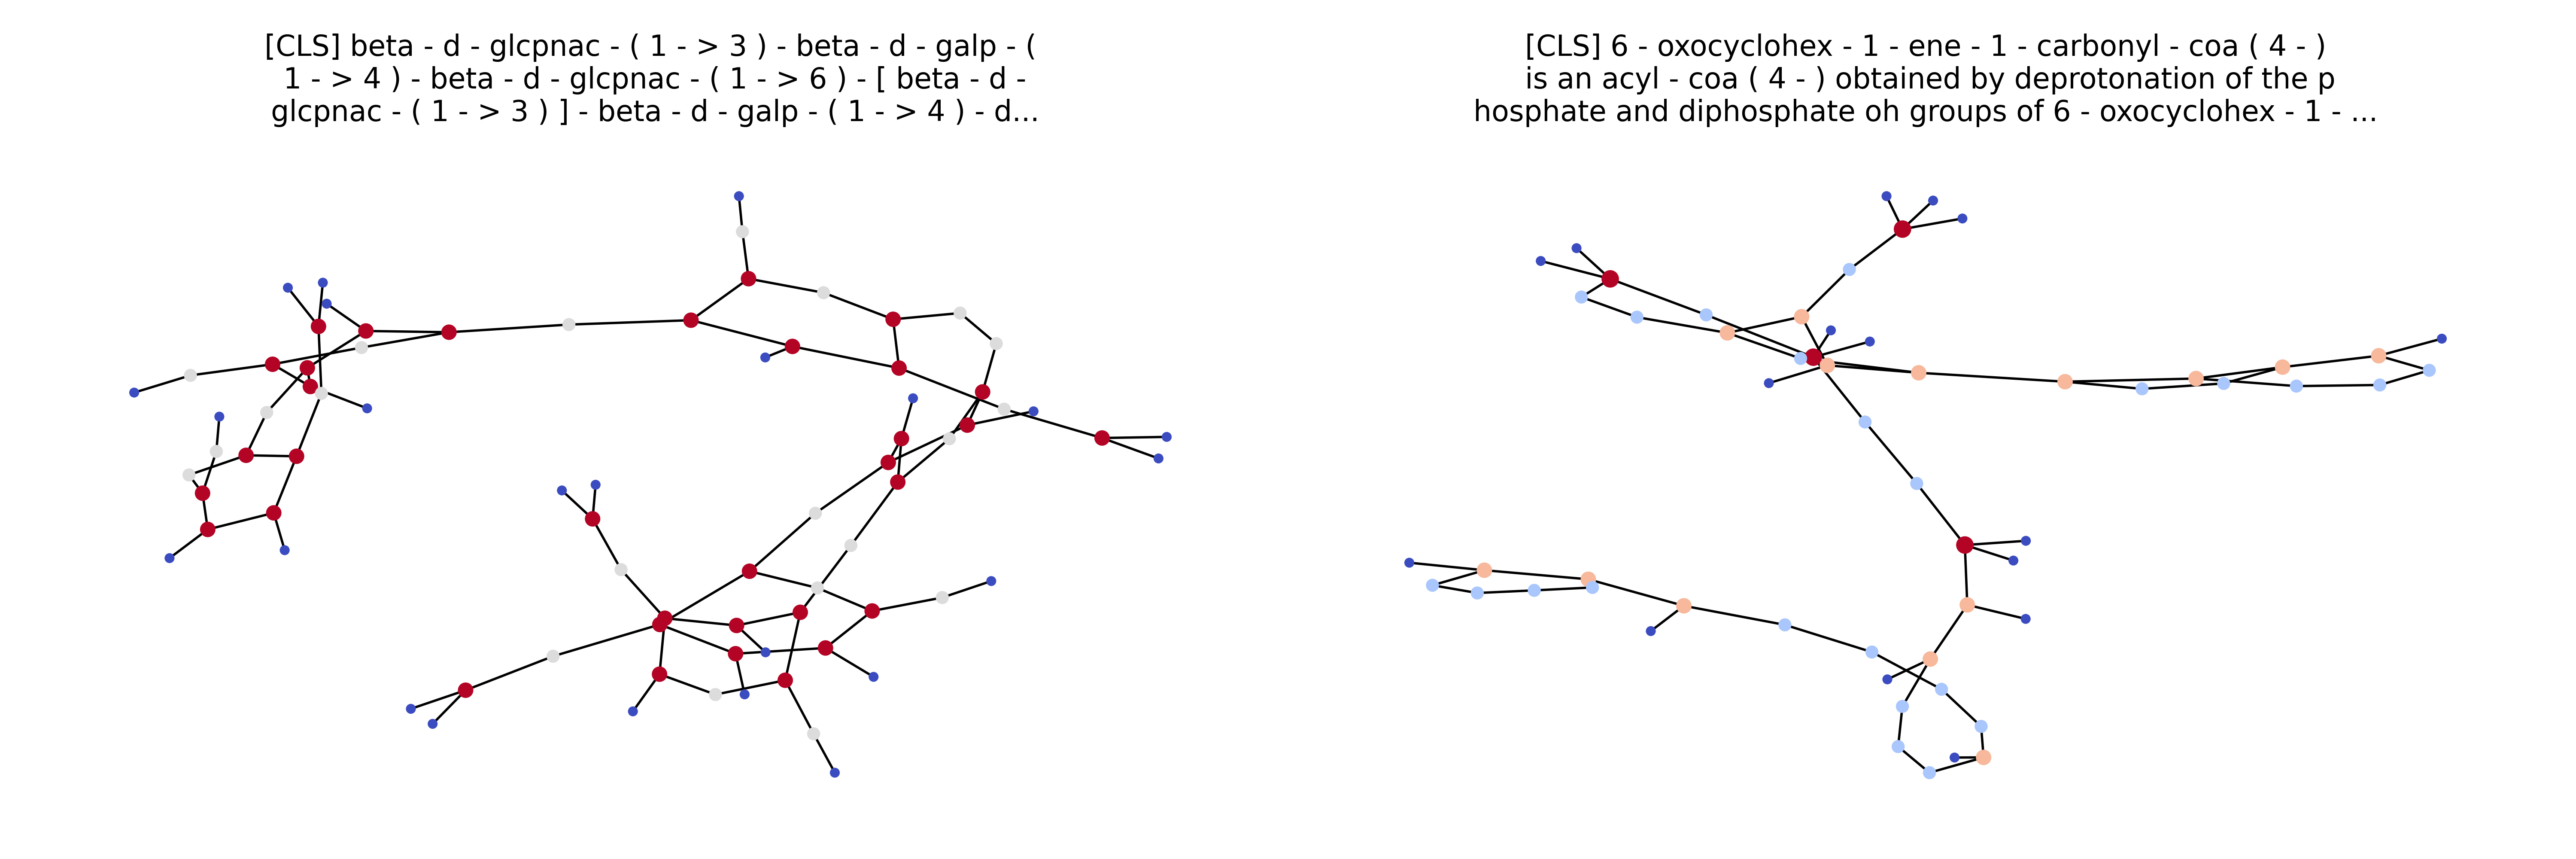
\includegraphics[width=\columnwidth]{figures/graphs.png}
        \caption{Two samples from the dataset.}
        \label{fig:dataset}
    \end{figure}

    The molecule descriptions are quite long, with some descriptions as long as 1500 characters. Realistically, we know that some of the longer descriptions are cut off, as the language models we used have a maximum input length of 512 tokens. Furthermore, looking at the tokenization of the descriptions, it's clear that they are not optimal for the language models, as a lot of words are cut in multiple tokens.

    The graphs are quite large, with the number of nodes ranging from 1 to 536 and a mean of 32. The number of edges is similarly distributed. The graph diameter is also quite large, with a maximum of 218 ! This is important when designing message passing models, as the number of message passing layers has to be chosen in accordance with the diameter of the graph.

    \section{Method}

    In this section, we describe the different models we used to encode the text and the graph. The text encoder and graph encoders are two separate models that are trained jointly using contrastive learning, so that they share the same embedding space.

    \subsection{Graph Attention Networks}

    Graph Attention Networks (GAT) \cite{velickovic-2018} have been shown to be effective in many tasks. Like other graph neural networks, GATs aggregate information from the neighbors of each node to compute its embedding. The main difference with other models is that GATs use an attention mechanism to weight the neighbors of each node. Specifically we used the improved version of GATs suggested in \cite{brody-2021}.

    Let $G$ be an undirected graph with $N$ nodes denoted $\llbracket1, N\rrbracket$. Let $d$ be the dimension of the node embeddings, and $h_1,\dots,h_N\in\R^d$ be the said embeddings. Let $W\in\R^{d'\times d}$ and $a\in\R^{2d'}$. The attention weights are :
    \begin{equation}
        e(h_i,h_j) = a^T \leakyrelu([Wh_i || Wh_j])
    \end{equation}
    where $||$ denotes the concatenation operator. The attention weights are normalized using the softmax operator :
    \begin{equation}
        \alpha_{ij} = \frac{\exp(e(h_i,h_j))}{\sum_{k\in\mathcal{N}_i}\exp(e(h_i,h_k))}
    \end{equation}
    where $\mathcal{N}_i$ denotes the set of neighbors of node $i$ in $G$. This mechanism clearly allows the batch processing of graphs with different sizes. The embedding of node $i$ is then computed as :
    \begin{equation}
        h_i' = \leakyrelu\left(\sum_{j\in\mathcal{N}_i}\alpha_{ij}Wh_j\right)
    \end{equation}
    In general we will use multi-head attention, with $K$ heads, $a^{(1)},\dots,a^{(K)}\in\R^{2d'/K}$ and $W^{(1)},\dots,W^{(K)}\in\R^{d'/K\times d}$ :
    \begin{equation}
        h_i' = \leakyrelu\left(\frac{1}{K}\sum_{k=1}^K\sum_{j\in\mathcal{N}_i}\alpha_{ij}^{(k)}W^{(k)}h_j\right)
    \end{equation}
    Furthermore, we will stack multiple GAT layers to obtain a deeper model. We may also apply a multi-layer perceptron to the embeddings of the last layer to obtain a more expressive representation.


    \subsection{DiffPool}
    A limitation of Graph Neural Networks (GNNs) is the inherently flat structure of the embeddings. This means that the more macroscopic structure of the graph is not very well captured, since these structural aspects are only encoded by the very local message passing layers. GATs, as we have seen, are designed to capture a more nuanced version of these local structures since they use an attention mechanism to weight the neighbors of each node. However, the global structure of the graph is still not very well captured, even when exploring larger radius neighborhoods.

    DiffPool \cite{ying-2018} is a method that aims to address this issue. It is a differentiable graph pooling layer that can be used to learn a hierarchical representation of the graph. The main idea is to learn a set of cluster assignments as well as new embeddings for the nodes, and then to use these assignments and embeddings to coarsen the graph. The coarsened graph is then passed to another GNN, and the process is repeated until the graph is small enough. The embeddings of the nodes in the last layer are then used as the graph embedding.

    Let's briefly describe the two main steps of the DiffPool algorithm. We will denote
    \begin{enumerate}
        \item \textbf{Cluster assignment and new embeddings (GAT layers)} : In the original paper \cite{ying-2018}, the cluster assignments as well as the new embeddings are learned using GNNs. However, in our case, we will use GATs. This allows for a more expressive representation of the nodes.

              More specifically, the new embeddings at layer $(l)$ are denoted $Z^{(l)}\in\R^{n_l\times d}$, and are simply obtained as the output of a GAT,
              $$Z^{(l)} = \text{GAT}_{l, \text{ embed}}\left(A^{(l)},X^{(l)}\right).$$
              \noindent The cluster assignments at layer $(l)$ are denoted $S^{(l)}\in\R^{n_l\times n_{l+1}}$, and are obtained by applying a softmax function to the output of another GAT (with independent parameters),
              $$S^{(l)} = \text{softmax}\left(\text{GAT}_{l, \text{ pool}}\left(A^{(l)},X^{(l)}\right)\right).$$
              \noindent As we can see from the last equation, the cluster assignments are a probability distribution over the nodes of the graph. This means that the cluster assignments are soft, and that each node can belong to multiple clusters.
        \item \textbf{Graph coarsening (Diffpool layer)} : The coarsened graph is obtained by simply applying the cluster assignments to the new computed embeddings. More specifically, the adjacency matrix of the coarsened graph $A^{(l+1)} \in \R^{n_{l+1}\times n_{l+1}}$ is obtained as
              $$A^{(l+1)} = {S^{(l)}}^TA^{(l)}S^{(l)}.$$

              The new node embeddings $X^{(l+1)}\in\R^{n_{l+1}\times d}$ are obtained as
              $$X^{(l+1)} = {S^{(l)}}^T Z^{(l)}.$$
    \end{enumerate}
    At the end of the process, a multi-layer perceptron is typically applied to the embeddings of the last layer.

    We can therefore see that a series of coarsening steps are applied to the graph, which results in a smaller graph that captures the global structure of the original graph. Figure \ref{fig:diffpool} that we have taken from the original paper \cite{ying-2018} with slight modifications illustrates the process.

    \begin{figure}[H]
        \centering
        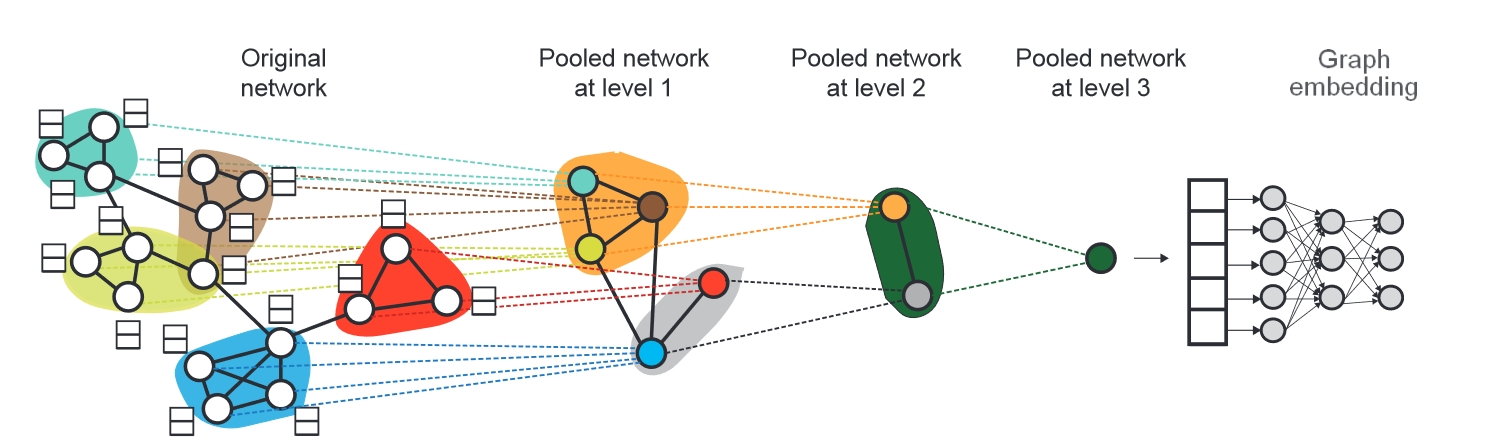
\includegraphics[width=0.5\textwidth]{figures/diffpool.jpg}
        \caption{Illustration of the DiffPool method taken from \cite{ying-2018}. The last feedforward neural network is used to obtain the graph embedding.}
        \label{fig:diffpool}
    \end{figure}
    Ying et al. have also shown in [Proposition 1, \cite{ying-2018}] that the permutation invariance of the DiffPool method is guaranteed, which is a crucial property for graph embedding methods.
    \subsection{Language modelling}

    We used a pretrained large language model (LLM) to encode the text. Specifically, we settled on \texttt{sentence-transformers/all-MiniLM-L6-v2} which is a distilled version of MiniLM \cite{wang-2020} known for its efficiency and relatively small size. The sentence embeddings are obtained by averaging the embeddings of the tokens in the sentence, which yields a 384-dimensional vector.

    \subsection{Ensembling}

    To improve the performance of our models, we used an ensemble of models. The idea is to train multiple models with different architectures and hyperparameters, and then fuse their predictions. The task of fusing rankings from multiple sources has been extensively studied in the context of recommendation systems \cite{bachanowski-2023}.

    Let's denote $s_1^{(i)}, \dots, s_N^{(i)}\in\R^N$ the similarities between the queries and the samples for the $i$-th model, and suppose we have $K$ models in our ensemble. The first thing we did was to normalize these similarities so that we can compare them. Quite surprisingly, we obtained the best results when using the following normalization accross queries :
    \begin{equation}
        \forall i\in \llbracket1, K\rrbracket, \forall j,k, \quad s_{j,k}^{(i)'} = \frac{s_{j,k}^{(i)} - \min_{l=1}^N s_{l,k}^{(i)}}{\max_{l=1}^N s_{l,k}^{(i)} - \min_{l=1}^N s_{l,k}^{(i)}}
    \end{equation}
    We also experimented with other normalization methods, such as min-max norm, rank norm, sum norm, max norm and ZMUV norm.

    After normalization, we used a simple weighted average to fuse the similarities :
    \begin{equation}
        s_{j,k} = \frac{1}{K}\sum_{i=1}^K w_i s_{j,k}^{(i)}
    \end{equation}
    Once again we experimented with different state of the art unsupervised fusion methods, such as Condorcet fusion \cite{montague-2002} and reciprocal rank fusion \cite{cormack-2009} which did not yield better results than the simple weighted average.

    The weights $w_1,\dots,w_K$ can be effectively chosen using the known performance of the models on the validation set. However we devised a more sophisticated method to choose the weights. We started with a simple grid search to find a good starting point for the weights, and then used an optimization algorithm to find the weights that maximized the LRAP on the validation set. We did not explore the possibility of differentiating the LRAP with respect to the weights, and instead settled on the Powell method \cite{powell-1964} which is a derivative-free optimization algorithm.

    Since we optimized the weights on the validation set, we thought this simple weighted average would avoid overfitting the weights to the validation set. In practice, we found that we did overfit a bit and so we submitted different solutions with different weights to the leaderboard to find some weights that generalize well.


    \section{Training}

    \subsection{A little history of our progression}
    Throughout the challenge, we tried different models and training procedures. In the following table, we summarize the main characteristics of the models we used and the scores we obtained.

    \begin{table}[H]
        \begin{center}
            \resizebox{\columnwidth}{!}{
                \begin{tabular}{|c|c|c|c|c|}
                    \toprule
                    \textbf{Text Encoder} & \textbf{Graph Encoder} & \textbf{Main characteristics} & \textbf{Score} \\
                    \midrule
                    BERT                  & GAT                    &                               & 0.5            \\
                    MiniLM-L6             & GAT                    &                               & 0.6            \\
                    MiniLM-L6             & GAT                    & Fine-tuned architecture       & 0.7            \\
                    MiniLM-L6             & DiffPool               &                               & 0.8            \\
                    MiniLM-L6             & DiffPool               & Fine-tuned architecture       & 0.86           \\
                    MiniLM-L6             & Ensemble               & Uniform weights               & 0.92           \\
                    MiniLM-L6             & Ensemble               & Fine-tuned weights            & 0.94           \\
                    \midrule
                \end{tabular}
            }
        \end{center}
        \caption{Model evolution throughout the challenge.}
    \end{table}

    We focused mainly on the graph encoder, as we thought that the text encoder was already quite sufficiente. The main improvement to the text encoder was to switch from BERT to MiniLM-L6, which is a smaller and faster model, with similar performance. This allowed us to train our models for longer and to use larger batch sizes.

    \subsection{Loss Function}

    Initially we used a cross-entropy loss to train the models. However, after some experimentation, we found that the circle loss \cite{sun-2020} resulted in faster training and better asymptotic performance.

    Consider a set of $N$ training samples, which results in $K=2N$ embeddings of dimension $d$ once passed through our model. There are $N$ pairs of positive embeddings (text and graph embeddings of the same molecule) and $L=N(N-1)$ pairs of negative embeddings. We chose the normalized cosine similarity as the similarity measure, so that the similarity between two embeddings $x$ and $y$ is defined as :
    \begin{equation}
        s(x,y)=\frac{x^Ty}{\|x\|\cdot\|y\|}
    \end{equation}
    We can thus denote $s_p^1,\dots,s_p^{2N}$ the similarities between the positive pairs and $s_n^1,\dots,s_n^{N(N-1)}$ the similarities between the negative pairs. The circle loss is defined as :
    \begin{align*}
        \mathcal{L}=\log\left[1+\sum_{j=1}^{L}\exp(\gamma\alpha_{n}^{j}(s_{n}^{j}-\Delta_{n}))\times \right. \\ \left.\sum_{i=1}^{K}\exp(-\gamma\alpha_{p}^{i}(s_{p}^{i}-\Delta_{p}))\right]
    \end{align*}
    where $\gamma$ is a scaling factor, $\alpha_{n}^{j}$ and $\alpha_{p}^{i}$ are linear weights for the negative and positive pairs, and $\Delta_{n}$ and $\Delta_{p}$ are the margins for the negative and positive pairs.

    \subsection{Training Procedure and implementation details}
    We mainly used the PyTorch library to implement the models. Let's detail in the following the main implementation details of the models.
    \paragraph*{DiffPool implementation for batch processing: } We can easily batch process graphs with different sizes using the DiffPool method. [TODO]

    \paragraph*{Optimizers and Learning Rate Schedulers: } We mainly used the Adam optimizer with a starting learning rate of $10^{-4}$.
    To automatically decrease the learning rate, we used a scheduler. More specifically, we fixed the learning rate to $10^{-4}$ for the first 10 epochs, and then decreased it by a factor of 0.05 at every epoch until the 100th. We then fixed the learning rate to the value it had at epoch 100 for the rest of the training.

    \paragraph*{Freezing and Unfreezing}
    We used a two-step training procedure. We first trained the graph encoder for 5 epochs with the text encoder frozen. After that, we trained the whole model for 100 epochs. This allowed the graph encoder to learn a good representation of the graphs before the text encoder starts to learn and gave noticeable improvements in the results and convergence speed.

    However, as will be further discussed in the results section, this freezing and unfreezing procedure has to be handled with care, as it can lead to very bad results if the freezing is too long while an ADAM optimizer is used. This is due to the fact that the moving averages of the gradients are updated with biased estimates of the gradients during the frozen phase.



    \footnotetext[1]{MPL: Message Passing Layer, the dimensions of the messages in the GNNs}
    \footnotetext[2]{The dimensions of the linear layers after the GNNs}
    \footnotetext[3]{Number of attention heads in each GAT layer}
\end{multicols}

\begin{table}[H]
    \begin{center}
        \resizebox{\columnwidth}{!}{
            \begin{tabular}{|c|c|c|c|c|c|c|c|c|c|}
                \toprule
                \textbf{Model name} & \textbf{DiffPool layers} & \textbf{MPL dimension}\footnotemark & \textbf{MPL} & \textbf{Linear layers}\footnotemark      & \textbf{Attention heads}\footnotemark & \textbf{Final linear layer} & \textbf{Graph parameters} & \textbf{Validation score} \\
                \midrule
                GAT                 & -                        & $1200$                              & $3$          & $[1200, 600]$                            & $6$                                   & -                           & $8\:891\:784$             & $0.6843$                  \\
                Diffpool-deep       & $15, 10, 5, 1 $          & $600, 600, 600, 600$                & $4, 3, 2, 2$ & $4\times[150, 150, 150]$                 & $4\times 3$                           & $700$                       & $14\:778\:965$            & $0.8367$                  \\
                Diffpool-old        & $10, 4$                  & $2 \times 600$                      & $2\times3$   & $2\times [1000, 500]$                    & $2\times 3$                           & $600$                       & $39\:671\:098$            & $0.8396$                  \\
                DiffPool-big        & $30, 10, 3, 1 $          & $300, 600, 1200, 1200$              & 10, 5, 3, 1  & $[300], [600], [1200, 600], [1200, 600]$ & $3, 6, 12, 12$                        & $1200$                      & $35\:616\:428$            & $0.8430$                  \\
                Diffpool-shallow    & $20, 3$                  & $2 \times 1200$                     & $4, 3$       & $2\times [150, 150, 150, 150]$           & $2\times 5$                           & $2000$                      & $34\:228\:057$            & $0.8462$                  \\
                DiffPool-base       & $15, 5, 1 $              & $3 \times 600$                      & $3, 3, 2$    & $3 \times [300]$                         & $3\times 3$                           & $1000$                      & $11\:454\: 805$           & $0.8515$                  \\
                Diffpool-medium     & $15, 5, 1 $              & $3 \times 600$                      & $6, 4, 3$    & $3\times [600, 300]$                     & $3\times 6$                           & $1200$                      & $20\:991\:405$            & $0.8716$                  \\
                Diffpool-linear     & $15, 5, 1 $              & $3 \times 600$                      & $4, 3, 2$    & $3\times [300, 300]$                     & $3\times 3$                           & $1200$                      & $13\:580\:805$            & $0.8804$                  \\
                Diffpool-large      & $15, 5, 1 $              & $3 \times 1200$                     & $5, 3, 2$    & $3\times [1200, 600]$                    & $3\times 6$                           & $1200$                      & $59\:116\:305$            & $0.8932$                  \\
                \midrule
            \end{tabular}
        }
    \end{center}
    \label{tab:models}
    \caption{Models hyperparameters.}
\end{table}
\begin{multicols}{2}
    \section{Results}
    \subsection{Results per trained model and discussion}
    We present on table \ref{tab:models} a detailed summary of the models we trained and the scores we obtained on the validation set. It has to be noted that all the models were trained with the same text encoder, which is a pretrained MiniLM-L6 model. As we can also see, all the models used a GAT-layered DiffPool model as the graph encoder, except for the first model which used a simple GAT model. This last model is also the one that yielded the worst results.

    A striking observation is that we obtained the best results with the DiffPool-large model, which is the model that has, by far, the most parameters. While this result is not surprising knowing the scalability of such models, it is still interesting to note that, in all the other models, the number of parameters seems to be unrelated to the performance of the model. More specifically, the DiffPool-linear model, which is one of the smallest models, yielded the second best results.

    These observations clearly emphasize the importance of the architecture of the model, and, by extension, the importance of the hyperparameter-tuning process. Nevertheless, because of the large number of hyperparameters, the considerable training time of the models, and our limited computational resources, we were not able to perform a thorough hyperparameter optimization process using raytune.

    An interesting observation that can be made from the results is that there doesn't seem to be a clear emerging pattern in the results, from which we could infer good guidelines for the design of the models. For example, the Diffpool-shallow model yielded better results than the Diffpool-deep model. This is quite surprising, as we would expect a deeper model to capture more complex structural information.


    \subsection{Global results after ensembling}
    \subsection{Execution time}

    \section{Other non-conclusive approaches}
    \label{sec:non-conclusive}
    \subsection{Other tested graph encoders}
    We tested other graph encoders ranging from relatively simple ones such as Graph Convolutional Networks (GCN) \cite{gcn}  and GraphSAGE \cite{graphsage} to more complex ones such as Graphormers \cite{graphormers} and PathNN \cite{pathnn}. We briefly describe the main characteristics of these last two models in the following as well as discuss the results we obtained.
    \begin{enumerate}
        \item \textbf{Graphormers: } Graphormers are a class of graph neural networks that are based on transformers. The main idea is to incorporate, beyond the information contained in the node features,  the structural insights of the graph into the attention mechanism of the transformer. Two encoding strategies from the ones proposed in the original paper \cite{graphormers} were jointly tested, namely the "Centrality Encoding" and the "Spatial Encoding".
        \item \textbf{PathNN: } PathNN \cite{pathnn} is a new class of graph neural networks that are based on the idea of aggregating information from paths starting from a node. The main idea is to go beyond the simple aggregation of the neighbors of a node, and to instead capture more complex structural information.
    \end{enumerate}
    Despite the interesting conceptual design of these models, the GAT-layered DiffPool model was the one that yielded the best results on the tests we conducted and on this particular dataset. We think that the main reason for this is that the GAT-layered DiffPool model is able to capture both the local and global structure of the graph, and that this is particularly important in the context of this challenge.
    \subsection{Language model fine-tuning}
    As mentioned before, we used a pretrained language model to encode the text. A natural track to follow is to fine-tune it on our specialized dataset. The idea is that since the starting pretrained language model was trained on a large corpus of text, the semantic information concerning the field of molecular chemistry was most likely completely undifferentiated, therefore lending very similar embeddings to very different molecules. Fine-tuning it on our dataset would allow the language model to learn a more specialized representation of the text, and therefore would yield better results.

    We tried to fine-tune the \texttt{bert-base-uncased} model that was pretrained on English Language text using a masked language modeling (MLM) objective. We simply did so by using an MLM objective, masking each time $15\%$ of the tokens of the text. We used an ADAMW optimizer with a learning rate of $5\times 10^{-5}$.

    Despite a model that seemed to be converging during the fine-tuning phase, we did not obtain any significant improvement in the results. We think that, in this particular case, the embeddings of the text using the pretrained language model were already sufficient to differentiate, throughout the training of the main model, the different molecules. We however still believe that fine-tuning the language model could lead to promising results if done differently.
    \subsection{Alternate training procedures}
    Among the numerous training procedures we tried, we can mention a few alternate training procedures that did not yield very promising results despite their conceptual appeal. We will briefly describe $2$ of these procedures in the following.
    \begin{enumerate}
        \item \textbf{Alternate freezing and unfreezing: } We tried to alternate the freezing and unfreezing of the text encoder and the graph encoder throughout the epochs, starting with a frozen text encoder and a trainable graph encoder, and then repeatedly switching the freezing of the two encoders. The hope was that this would allow the two parts to complement each other's training and result in a more balanced model.

              However, this procedure did not yield good results: the model steadily converged to a $0.5$ score on the validation set, but then started to decrease in performance and ended up oscillating around a $0.5$ score.

              We think that this is due to the fact that, while the text encoder is frozen (and vis-versa), the graph encoder is forced to take sub-optimal embedding optimization steps in directions that are not optimal for the final model. From step to step, the encoders try to independently move towards each other, but in a "selfish" fashion that do not lead to a good compromise between the two modalities.
        \item \textbf{Initial freezing of the text encoder: } This procedure is actually very efficient, and is the one we used in the final model. However, we want to emphasize here that an initial freezing of the text encoder has to be handled with care and balance. In one of our tests, we tried to freeze the text encoder until the score on the validation set reached a $0.5$ score threshold (which took about $30$ epochs), and then unfreeze the text encoder. We also made sure to use an SGD optimizer to avoid the problem of the moving averages of the gradients being updated with biased estimates of the gradients during the frozen phase.

              We found that this procedure led to very poor results with the model oscillating around a $0.5$ score on the validation set. The text encoder was not able to recover from the frozen phase. Our interpretation is actually the same as in the previous procedure. The text encoder was frozen for too long, and the graph encoder shifted its representation too far from the optimal compromise between the two modalities.

    \end{enumerate}

    \newpage

    \bibliography{bibliography}

\end{multicols}

\end{document}
